\section{Phase 3: Scalability and Load Balancing}\label{sec:phase3}

\subsection{Architecture}
Fig.~\ref{fig:arch3} adds two replicas and a load balancer (LB) to Fig.~\ref{fig:arch}.
The three servers are identical and keep no state per client; they share the corpus
and the Redis cache. Any replica can therefore answer any request, a count computed
by one replica is a cache hit for the others, and the hot keywords are counted over
all replicas. Clients only know the LB, which listens on the same port as a server.
The LB is a TCP proxy written with asyncio: for every client connection it chooses a
server, opens a connection to it and copies the bytes in both directions without
looking at the RPyC messages. Because it chooses per connection, the client opens a
new connection for every request.

\begin{figure}[t]
\centering
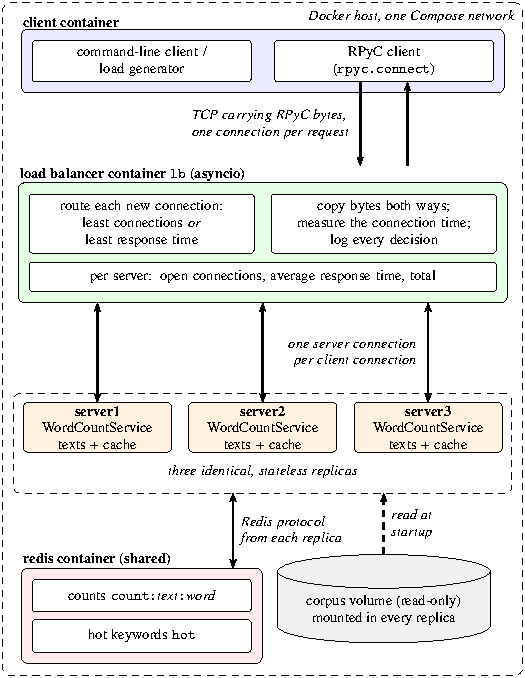
\includegraphics[width=\columnwidth]{figures/architecture_phase3}
\caption{Phase 3 architecture: the load balancer forwards each client connection to
one of three identical server replicas, which share one Redis cache.}
\label{fig:arch3}
\end{figure}

\subsection{Need for a Load Balancer}
In Phase~2 the tail latency of one server grew quickly from about
\textbf{[R]}\,req/s on, because all requests are processed one after another. More
servers only help if the requests are spread over them, and clients should not
have to know how many servers there are or which one is busy: they need a single
access point. A static split, such as sending requests to the servers in turn, does
not look at the load. Requests differ a lot in cost (a cache hit versus counting in
the largest book), so a server that received a few expensive requests keeps getting
its share and builds a queue while others are idle. A dynamic LB uses the current
state of the servers for every decision. The price is an extra hop for every request,
and the LB becomes a single point of failure.

\subsection{Algorithm 1: Least Connections}
Each new connection goes to the server with the fewest open connections. When
several servers have the same number, the one that was used longest ago is chosen,
so idle servers take turns. The LB keeps a counter per server that it increments when
it forwards a connection to that server and decrements when the connection closes.
Since every client connection carries one request, the counter is the number of
requests the server is currently handling.

\subsection{Algorithm 2: Least Response Time}
Least response time combines the response time of a server with its number of
active connections~\cite{aws_lb}: the LB chooses the server with the lowest
$(n_i+1)\cdot\bar r_i$, where $n_i$ is the number of open connections of server~$i$
and $\bar r_i$ its average response time. The $+1$ makes the response time decide
between idle servers. The LB measures the response time as the duration of each
connection it forwards and keeps a moving average
($\bar r \leftarrow 0.9\,\bar r + 0.1\,r$). A server that was not used in the last
second counts as 0, so it is tried again: in testing, a server that was slow once
was otherwise never chosen again, so its average was never updated.

\subsection{Experiments}
We use the setup of Table~\ref{tab:setup} with three servers. (a)~\emph{Distribution}:
the LB logs one line per connection with the chosen server, the numbers the
algorithm used (the open connections, or the score $(n_i+1)\cdot\bar r_i$) and the total
number of connections per server
(Figs.~\ref{fig:shot-lc} and~\ref{fig:shot-lrt}); the load generator also records
which server answered each request. (b)~\emph{Latency}: the same requests at the same
rates as in Phase~2, three runs per rate, once through the LB with each algorithm,
compared with one server without LB (Figs.~\ref{fig:mean3} and~\ref{fig:p99-3}).

\subsection{Results}
% TODO after the runs: replace the bracketed values and keep only what your data shows.
\emph{Distribution.} With least connections every server answered about a third of
the requests (\textbf{[shares]}). In Fig.~\ref{fig:shot-lc} most connections find all
servers idle, so the servers take turns; under load, a server with more open
connections is skipped until it catches up. Least response time is uneven: at
\textbf{[R1]}\,req/s \textbf{[serverX]} answered \textbf{[y]}\% of the requests because
its measured response time was the lowest (Fig.~\ref{fig:shot-lrt}); at higher rates
the factor $(n_i+1)$ spreads the requests more (\textbf{[shares at R5]}). Since the
servers are identical, these differences mostly depend on which requests a server
happened to get, e.g., cache misses on large books.

\emph{Latency.} At \textbf{[R1]}\,req/s three servers are \emph{slower} than one, by
\textbf{[d]}\,ms on average: every request passes an extra TCP hop and the LB copies
all its bytes, while a single server was not busy enough yet to profit from more
servers. At \textbf{[R5]}\,req/s the 99th percentile of one server reaches
\textbf{[c]}\,ms, while with three servers each one handles a third of the load and the
99th percentile stays at \textbf{[e]}\,ms. \textbf{[Which algorithm had the lower tail
and why]}: least connections reacts directly to waiting requests, while least
response time sends more requests to the server it measured as fastest.

\begin{figure}[t]
\centering
\includegraphics[width=\columnwidth]{figures/screenshot_lc}
\caption{LB log with least connections: each line is one connection with the chosen
server, the open connections per server, and the number of connections per server so far.}
\label{fig:shot-lc}
\end{figure}

\begin{figure}[t]
\centering
\includegraphics[width=\columnwidth]{figures/screenshot_lrt}
\caption{LB log with least response time: per server the score
$(n_i+1)\cdot\bar r_i$ used for the decision.}
\label{fig:shot-lrt}
\end{figure}

\begin{figure}[t]
\centering
\includegraphics[width=\columnwidth]{figures/phase3_mean}
\caption{Average latency: one server (Phase 2) and three servers with each algorithm
(average of 3 runs).}
\label{fig:mean3}
\end{figure}

\begin{figure}[t]
\centering
\includegraphics[width=\columnwidth]{figures/phase3_p99}
\caption{99th-percentile latency: one server (Phase 2) and three servers with each
algorithm (average of 3 runs).}
\label{fig:p99-3}
\end{figure}
